\StartOf{Lecture 13}

\Today{QAM/PSK Probability of Error: (1) Union Bound, (2) Nearest neighbor approximation}

\announcements{
\begin{itemize}
  \item Reading: today: Rice 6.2. Mon after break: Rice 7.7, Proakis-Salehi pages 423-427 (Section 7.6.6)
  \item Project 4 due today.
  \item HW 6 due Wed after break. (My mistake on original Canvas deadline.)
\end{itemize}
}


\section{QAM/PSK Probability of Error}



\subsection{Options for Probability of Error Expressions}

Here are some choices you have to compute the probability of error for particular modulations.  In order of preference:
\begin{enumerate}
 \item \textit{Exact formula}.  In a few cases, there is an exact expression for $\PR{\mbox{symbol error}}$ in an AWGN environment, e.g., for square QAM, for PAM, for PSK.
 \item \textit{Union bound}.  This is a provable upper bound on the probability of error.  It is not an approximation, in that sense.  It can be used for ``worst case'' analysis which is often very useful for the engineering design of systems.
 \item \textit{Nearest Neighbor Approximation}.  This is a way to get a solution that is analytically easier to handle.  Typically this approximation is good at high $\Ebno$.
\end{enumerate}



\subsection{Exact Error Analysis}

As we discussed last time, the exact probability of error formulas in $N$-dimensional modulations with arbitrary constellation diagrams can be very difficult to compute.  This is because our decisions regions are more complex than one threshold test.  They require an integration of a $N$-D Gaussian pdf across an area.  We needed a Q function to get a tail probability for a 1-D Gaussian pdf.  To find the probability of a subspace of $N$-D Gaussian pdf, we need not just a tail probability... but a $N$-D integral under some part of the $N$-dimensional pdf.

For example, consider $M$-ary PSK.
\begin{figure}[htbp]
  \centerline{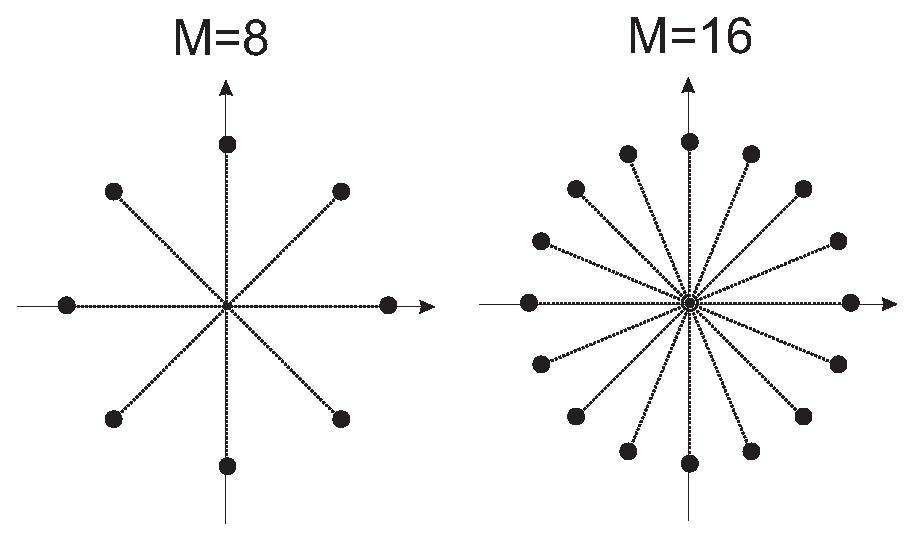
\includegraphics[width=0.5\textwidth]{../images/MPSK-signalSpaceDiagram.eps}}
  \caption{Signal space diagram for $M$-ary PSK for $M=8$ and $M=16$.}
  \label{F:MPSK-signalSpaceDiagram2}
\end{figure}
Essentially, we must find calculate the probability of symbol error
as 1 minus the area in the sector within $\pm \frac{\pi}{M}$ of the
correct angle $\phi_i$.  This is,
\begin{equation} \label{E:ExactMPSK-PE}
  P(\mbox{symbol error}) = 1 - \int_{r\in R_i} \frac{1}{2\pi \sigma^2} e^{-\frac{\| \mbr - \mbalpha_i \|^2}{2\sigma^2}}
\end{equation}
This integral is a double integral, and we don't generally have any
exact expression to use to express the result in general.


\subsection{Probability of Error in QPSK}
In QPSK, the probability of error is analytically tractable. Consider the QPSK constellation diagram, when Gray encoding is used. You have already calculated the decision regions for each symbol; now consider the decision region for the first bit. 

The decision is made using \emph{only} one dimension, of the received signal vector $\mbx$, specifically $x_1$. Similarly, the second bit decision is made using only $x_2$.  Also, the noise contribution to each element is independent.  The decisions are decoupled -- $x_2$ has no impact on the decision about bit one, and $x_1$ has no impact on the decision on bit two.  Since we know the bit error probability for each bit decision (it is the same as
bipolar PAM) we can see that the bit error probability is also
\begin{equation}\label{E:ExactQPSK_PBE}
  \PR{\mbox{error}} = \Q{ \sqrt{\frac{2\En_b }{N_0}}}
\end{equation}

This is an extraordinary result -- the bit rate will double in QPSK, but in theory, the bit error rate does not increase.  As we will show later, the bandwidth of QPSK is identical to that of BPSK.


\subsection{Neighbors}

For a particular symbol $i$ in a constellation, we define the concept of \emph{neighbors}.  These are the symbols $j$ which are necessary to draw the (Voronoi) decision region for symbol $i$.  That is, the perpendicular bisector of the line between $i$ and $j$ is one of the boundaries of the decision region for $i$.  We denote this set as $N(i)$.

The \emph{nearest neighbors} is the set of neighbors which are at the minimum distance $d_{i,j}$ for all $j$ in $N(i)$.  There may be several neighbors $j$ with exactly the same distance $d_{i,j}$, which is the reason the nearest neighbors is a set, but of course there is a minimum of one nearest neighbor of $i$.  We denote this set as $NN(i)$.

\Example{Listing Neighbor Symbols}

Consider the constellation in Figure \ref{F:ExampleVoronoiDiagramLabelledSolutions}.
\begin{enumerate}
\item What are the neighbors of 1, $N(1)$?
\item What are the nearest neighbors of 1, $NN(1)$?
\end{enumerate}

\Solution{ For (1), $N(1) = \{4,5,6,9,10\}$.  Note that 3 could be a neighbor, since we've only drawn the Voronoi boundaries within the $[0,1]^2$, and the line for $(10,3)$ may intersect with the line from $(1,10)$ far to the upper left of this figure.  For (2) just by looking at the plot, $NN(1)=\{4\}$.}

Generally, since we don't put symbols in random locations as was done for this plot, it is easier to define neighbors and nearest neighbors.

\begin{figure}[htbp]
  \centerline{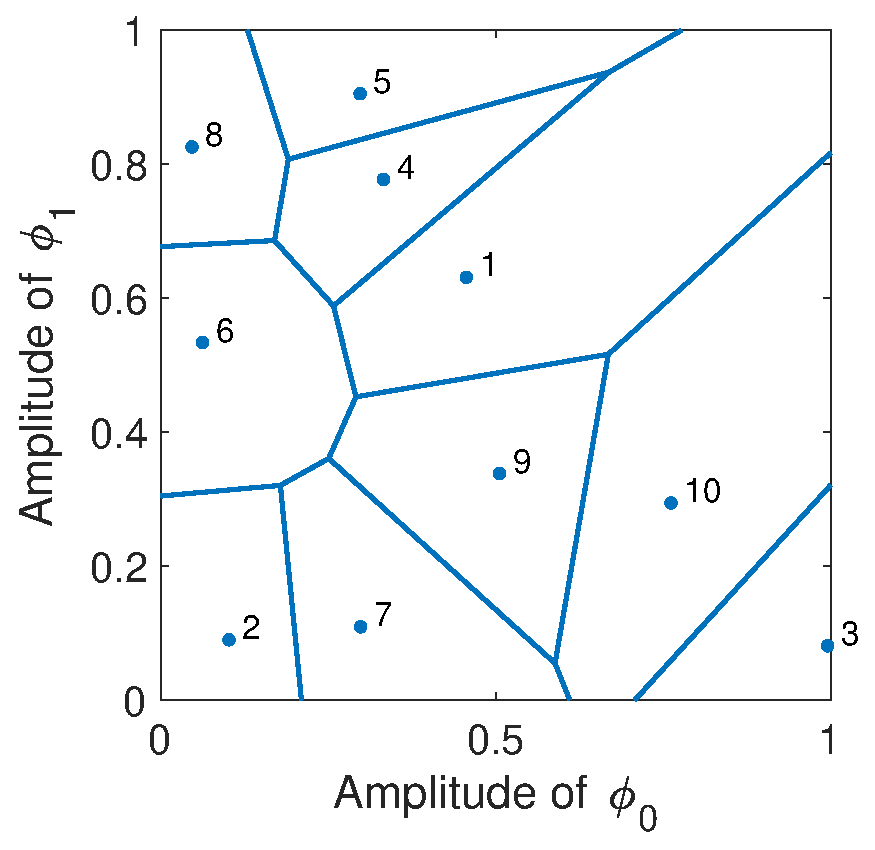
\includegraphics[width=0.8\textwidth]{../images/ExampleVoronoiDiagramLabelledSolutions.eps} }
  \caption{An example constellation diagram.  Find the neighbors and nearest neighbors of each symbol.  }
  \label{F:ExampleVoronoiDiagramLabelledSolutions}
\end{figure}


\subsection{Probability of $j|i$ Error}

What is the probability of deciding $H_j$ when $H_i$ is true?  When the space is divided into two, that is, there are no other symbols, this probability of being closer to $\mba_j$ than to $\mba_i$ can be computed with a 1-D integral of a Gaussian pdf.  Recall from probability that any linear combination of a multi-variate Gaussian vector is also Gaussian.  If we rotate the axes so that one is parallel to the line between $\mba_i$ and $\mba_j$ (which we call the \emph{new axis}, then this rotated vector is also multivariate Gaussian, and the distance along this new axis is Gaussian.  Further because the standard deviation is identical in every dimension, the standard deviation of the value on this new axis is also the same, $\sigma_W = \sqrt{N_0/2}$.  Let $y$ be the value along the new axis.

Consider the probability that, given $i$ was sent, that $y$ is closer to $j$ than to $i$ and thus we decide $H_j$.  Denote this event $E_{j|i}$.  Since $\mba_i$ and $\mba_j$ are $d_{i,j} = \| \mba_i - \mba_j\|$ apart, the threshold is halfway between, or  $d_{i,j}/2$ away from the $\mba_i$.  The probability is
\begin{equation} \label{E:RicePairwiseErrorPrep}
  \PR{E_{j|i}} = \Q{ 
  \frac{d_{i,j}/2}{\sqrt{N_0/2}}
  }
  = 
  \Q{
  \sqrt{\frac{d_{i,j}^2}{4}}\sqrt{\frac{2}{N_0}}
  }
  = 
  \Q{ 
  \sqrt{\frac{d_{i,j}^2}{2N_0}}
  }
\end{equation}

We often want the  \emph{pairwise probability of error} in terms of $\Ebno$ or $\En_s/N_0$.  To make this more explicit, I am also showing the first step in how to get this expression:
\begin{equation} \label{E:RicePairwiseError_a}
  \PR{E_{j|i}} = \Q{\sqrt{\frac{d^2_{i,j}}{2N_0}}}
  = \Q{\sqrt{\frac{d^2_{i,j}}{2\En_s}\frac{\En_s}{N_0}}}
  = \Q{\sqrt{\frac{d^2_{i,j}}{2\En_b}\frac{\En_b}{N_0}}}
\end{equation}
If we use a constant $A$ when describing the signal space vectors (as we usually do), then, since $\En_s$ will be proportional to $A^2$ and $d^2_{m,n}$ will be proportional to $A^2$, the factors $A$ will cancel out of the expression.

A more detailed proof of (\ref{E:RicePairwiseError_a}) is detailed in Section 6.2 of the Rice book.





\subsection{Union Bound}

From 5510 or an equivalent class (or a Venn diagram) you may recall
the probability formula, that for two events $E$ and $F$ that
\[
  \PR{E \cup F} = \PR{E} + \PR{F} - \PR{E \cap F}
\]
You can prove this from the three axioms of probability. (This holds
for \emph{any} events $E$ and $F$!) Then, using the above formula,
and the first axiom of probability, we have that
\begin{equation} \label{E:UnionBound2}
  \PR{E \cup F} \le \PR{E} + \PR{F}.
\end{equation}
Furthermore, from (\ref{E:UnionBound2}) it is straightforward to
show that for \emph{any} list of sets $E_1, E_2, \ldots E_n$ we have
that
\begin{equation} \label{E:UnionBound}
  \PR{ \bigcup_{i=1}^n E_i } \le \sum_{i=1}^n \PR{E_i}
\end{equation}
This is called the \emph{union bound}, and it is very useful across
communications.  If you know one inequality, know this one.  It is
useful when the overlaps $E_i \cap E_j$ are small but difficult to
calculate.  

\begin{figure}[htbp]
  \centerline{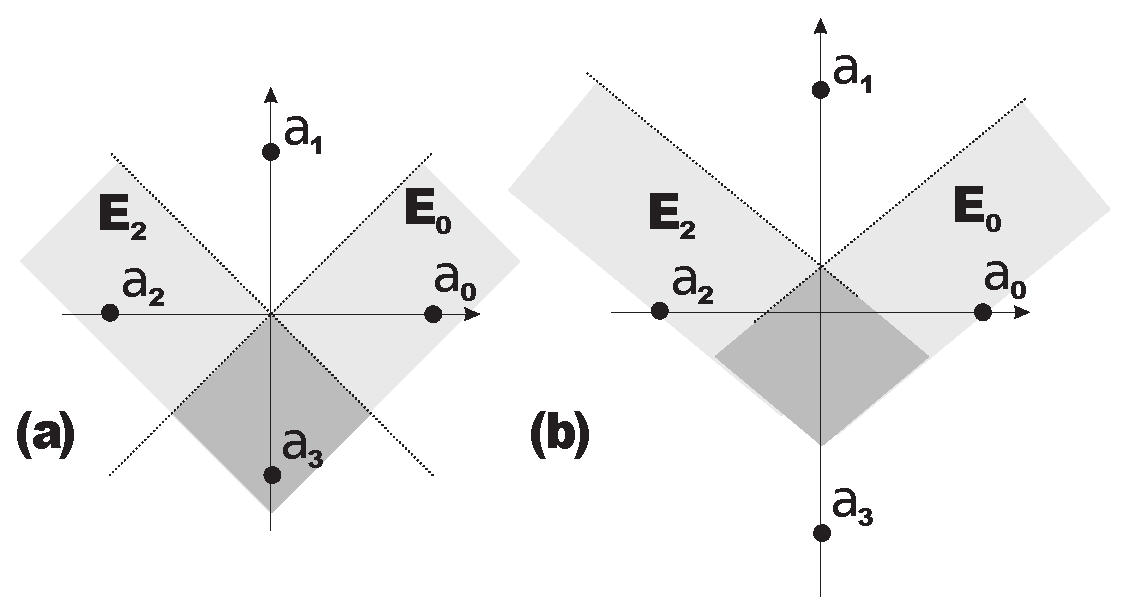
\includegraphics[width=0.7\textwidth]{../images/UnionBoundEg2.eps} }
  \caption{Union bound examples. (a) is QPSK with symbols of equal energy
    $\sqrt{\En_s}$.  In (b) $\mba_1 = -\mba_3 = [0, \sqrt{3\En_s/2}]^T$
    and $\mba_2 = -\mba_0 = [\sqrt{\En_s/2},0]^T$.  }
  \label{F:UnionBoundEg}
\end{figure}

\Example{QPSK}  First, let's study the union bound for QPSK, as
shown in Figure \ref{F:UnionBoundEg}(a).  Assume $s_1(t)$ is sent.
We know that from our previous lecture on square QAM:
\begin{equation} 
  P(\mbox{bit error}) \approx \frac{4(\sqrt{M}-1)}{\sqrt{M} \log_2 M} \Q{\sqrt{\frac{3 \log_2 M}{M-1} \frac{\En_b}{N_0}}}.
\end{equation}
For $M=4$, this result uses $\sqrt{M}=2$ and $\log_2 M = 2$, thus:
\begin{equation} \label{E:PrSymbolErrorMPAM_review}
  P(\mbox{bit error}) \approx \frac{4}{2 (2)} \Q{\sqrt{\frac{3 (2)}{3} \frac{\En_b}{N_0}}}.
\end{equation}
Or
\[
  \PR{\mbox{bit error}} = \Q{\sqrt{\frac{2 \En_b}{ N_0}}}
\]
The probability of symbol error is one minus the probability that there were no error in either bit,
\begin{equation}\label{E:UnionBoundEg1a}
  \PR{\mbox{symbol error}} = 1-\left(1-\Q{\sqrt{\frac{2 \En_b}{ N_0}}}\right)^2
\end{equation}
We can also write this as:
\begin{equation}\label{E:UnionBoundEg1b}
  \PR{\mbox{symbol error}} = 2\Q{\sqrt{\frac{2 \En_b}{ N_0}}} - \left[ 2\Q{\sqrt{\frac{2 \En_b}{ N_0}}}\right]^2
\end{equation}

In contrast, let's calculate the union bound on the probability of
error. There are two neighbors of each node $i$.  Consider for example node $i=1$.  We can write
\[
  \PR{\mbox{symbol error} | H_1} = \PR{E_2 \cup E_0}
\]
We ignored $E_3$ because it overlaps completely with $E_2 \cup E_0$.
That is, $E_2 \cup E_0 \cup E_3 = E_2 \cup E_0$.

Then, we use the union bound.
\[
  \PR{\mbox{symbol error} | H_1} \le  \PR{E_2} + \PR{E_0}
\]
These two probabilities are just the probability of error for a
binary modulation, and both are identical, so
\[
  \PR{\mbox{symbol error} | H_1} \le  2 \Q{\sqrt{\frac{2 \En_b}{ N_0}}}
\]

The overall probability of error is the average of $\PR{\mbox{symbol error} | H_i}$ for $i=0,1,2,3$; however these will all be identical due to the symmetry of QPSK.  Thus $\PR{\mbox{symbol error} } = \PR{\mbox{symbol error} | H_1}$.


What is missing / What is the difference in this expression compared
to (\ref{E:UnionBoundEg1b})?

See Figure \ref{F:PERPlotUnionBound} to see the union bound
probability of error plot, compared to the exact expression.  Only
at very low $E_b/N_0$ is there any noticeable difference!

\begin{figure}[htbp]
  \centerline{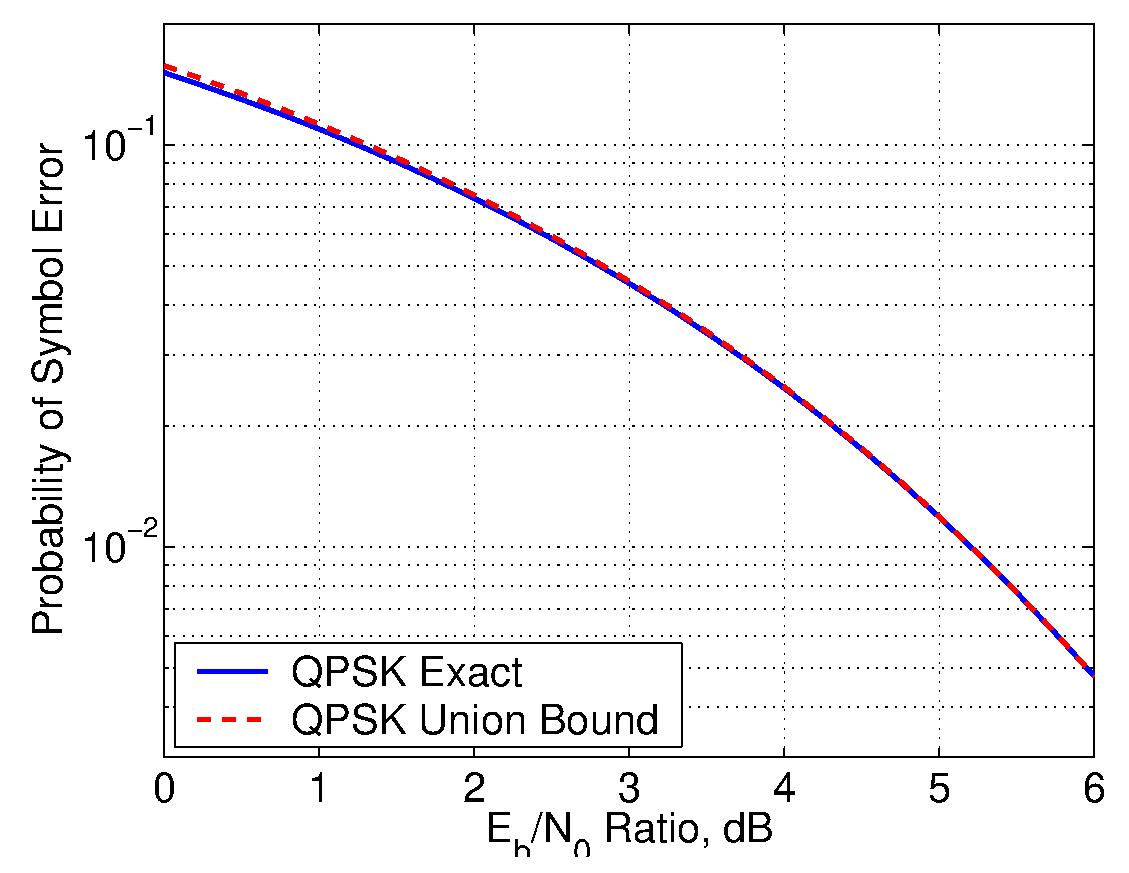
\includegraphics[width=0.75\textwidth]{../images/plotProbBitErrPSK_UnionBound.eps} }
  \caption{For QPSK, the exact probability of symbol error expression vs.\ the union bound.  }
  \label{F:PERPlotUnionBound}
\end{figure}


\subsection{General Application of Union Bound}

In this class, our events are typically error events.  Let $E_{j|i}$  represent the event that we decide $H_j$, when a different
symbol $i$ was actually sent.  In this case,  the union bound can be used to find the overall error given that $i$ was sent:
\begin{equation} \label{E:UnionBound_5}
  \PR{ \mbox{symbol error} | H_i } \le \sum_{j\in N(i)} \PR{E_{j|i}}
\end{equation}
These events $E_{j|i}$ for all $j\in N(i)$ cover all of the area outside of the decision region for $i$.  That is, by combining their $\PR{E_{j|i}}$, we are greater than or equal to the probability of error given symbol $i$ was sent.  

The overall probability of error, averaged over all $i$ that could be sent, is 
\begin{equation} \label{E:UnionBoundMid}
  \PR{ \mbox{symbol error} } \le \frac{1}{M} \sum_{i=0}^{M-1} \sum_{j\in N(i)} \PR{E_{j|i}} 
\end{equation}
Using the formula from (\ref{E:RicePairwiseError_a}),
\begin{equation} \label{E:UnionBound_applied}
  \PR{ \mbox{symbol error} } \le \frac{1}{M} \sum_{i=0}^{M-1} \sum_{j\in N(i)}  \Q{\sqrt{\frac{d^2_{i,j}}{2N_0}}}
\end{equation}

The union bound gives a conservative estimate.  This can be useful
for quick initial study of a modulation type.

\subsubsection{Rice book formula}
This is the formula for the Union bound given in Rice book:
\begin{eqnarray} \label{E:RiceUnionBound}
  \PR{\mbox{symbol error}} &\le & \frac{1}{M} \sum_{m=0}^{M-1} \sum_{n=0 \atop n\neq m}^{M-1} \PR{\mbox{decide } H_n | H_m}
 \nn
\end{eqnarray}
Note the $\le$ sign.  This means the actual $\PR{\mbox{symbol error}}$ will be \textit{at most} this value.  It is probably less than this value.  This is a general formula and \textit{is not necessarily the best} upper bound.  What do we mean?  If I draw any function that is always above the actual $\PR{\mbox{symbol error}}$ formula, I have drawn an upper bound.  But I could draw lots of functions that are upper bounds, some higher than others.

In particular, for some of the error events, decide $H_n | H_m$ may be redundant, and do not need to be included.  We have talked about the concept of ``neighboring'' symbols and ``nearest neighboring'' symbols to symbol $i$, which we call respectively, $N(i)$ and $NN(i)$.  The $N(i)$ are the ones that are necessary to include in the union bound.

Note that the Rice book uses $E_{avg}$ where I use $\En_s$ to denote
average symbol energy.  The Rice book uses $E_b$ where I use $\En_b$
to denote average bit energy. 



\Example{4-QAM with two amplitude levels}  This is shown (poorly) in
Figure \ref{F:UnionBoundEg}(b).  The amplitudes of the top and
bottom symbols are $\sqrt{3}$ times the amplitude of the symbols on
the right and left.  (They are positioned to keep the distance
between points in the signal space equal to $\sqrt{2\En_s/N_0}$.)  I
am calling this ``2-amplitude 4-QAM'' (I made it up).

What is the union bound on the probability of symbol error, given
$H_1$? 

\Solution{ Given symbol 1, the probability is the same as
above. Defining $E_2$ and $E_0$ as above, these two distances
between symbol $\mba_1$ and $\mba_2$ or $\mba_0$ are the same:
$\sqrt{2\En_s/N_0}$. Thus the formula for the union bound is the
same.}

What is the union bound on the probability of symbol error, given
$H_2$? \Solution{Now, it is
\[
  \PR{\mbox{symbol error} | H_2} \le  3 \Q{\sqrt{\frac{2 \En_b}{ N_0}}}
\]
}

So, overall, the union bound on probability of symbol error is
\[
  \PR{\mbox{symbol error} } \le  \frac{3\cdot 2 + 2\cdot 2}{4} \Q{\sqrt{\frac{2 \En_b}{ N_0}}} = 2.5 \Q{\sqrt{\frac{2 \En_b}{ N_0}}}.
\]

How about average energy? For QPSK, the symbol energies are all
equal.  Thus $\En_{av} = \En_s$.  For the two-amplitude 4-QAM
modulation,
\[
  \En_{av} = \En_s \frac{2(0.5) + 2(1.5)}{4} = \En_s
\]
Thus there is no advantage to the two-amplitude QAM modulation in
terms of average energy.





\subsection{Nearest-Neighbor Approximate Probability of Error}

As it turns out, the probability of error is often well approximated
by the terms in the Union Bound with the smallest
$d_{i,j}$.  This is because higher $d_{i,j}$ means a higher argument
in the Q-function, which in turn means a lower value of the
Q-function.  A little extra distance means a much lower value of the
Q-function.  So approximately,
\begin{eqnarray} \label{E:NearestNeighborApproximatePError}
  \PR{\mbox{symbol error}}  &\approx & \frac{N_{min}}{M}  \Q{\sqrt{\frac{d^2_{min}}{2N_0}}} \nn
\end{eqnarray}
where
\[
  d_{min} = \min_{j\neq i} d_{i,j}, \quad m,n \in \{0, \ldots, M-1\}
\]
and $N_{min}$ is the number of \emph{ordered pairs} of symbols which are separated by distance $d_{min}$.  Be sure to double count each pair, otherwise this formula won't work!

\Example{2-Amplitude 4-QAM}
What is the nearest neighbor approximation for 2-Amplitude 4-QAM?

\Solution{
The minimum distance $d_{min} = 2A  = \sqrt{2\En_s}$.  Starting from symbol 0, I count 3, 2, 3, and 2 such distances.  This is a total of $N_{min} = 10$.  Thus
\[
\PR{\mbox{symbol error}}  \approx  \frac{10}{4}  \Q{\sqrt{\frac{2\En_b}{N_0}}} \nn
\]
The same as the Union Bound.
}
